\section{Parallel Transport \& Curvature}
Parallel transport of a vector $Y$ along a curve $\gamma$ means $\nabla_{v_\gamma} Y = 0$,
where $v_\gamma$ is the tangent vector along $\gamma$.
As we see in figure~\ref{fig:parallelTransportSphere} if there is curvature,
then the vector we get actually depends on the path we take.
\begin{figure}[tbh]
    \centering
    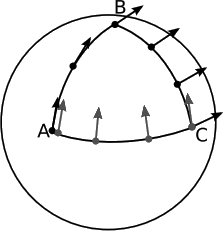
\includegraphics[width = 0.4\textwidth]{figures/parallelTransportSphere.png}
    %\includesvg[width = 0.4\textwidth]{figures/parallelTransportSphere}
    \caption{Parallel Transport on a sphere. Parallel transporting the vector along ABC gives
    a different vector than along AC. Figure from~\cite{parallelTransportFigure}}
    \label{fig:parallelTransportSphere}
\end{figure}

\subsection{Parallelity of Vector Fields}
Let $(\M, \mathcal{O}, \mathcal{A}, \nabla)$ a vector field with connection.
\begin{defn}[Parallel Transport]
    A vector field $X$ on $\M$ is said to be \textit{parallely transported} along a smooth curve $\gamma: \mathbb{R}\to \M$
    if 
    \begin{equation}
        \boxed{
        \nabla_{v_\gamma} X = 0\,.
    }
    \end{equation}
    Another way of writing this is
    \begin{equation}
        \left(\nabla_{v_{\gamma, \gamma(\lambda)}}X\right)_{\gamma(\lambda)}\,,\quad\forall \lambda
    \end{equation}
\end{defn}
\begin{note}
    $v_\gamma$ is not a vector field, but a vector at each point of the curve.
    Here it is actually important that the derivative $\nabla_Y X$ only needs a
    vector field $X$ and a vector $Y$ at the point where the derivative is taken!
\end{note}

\begin{defn}[Parallel]
    A vector $X$ is said to be parallel along the curve $\gamma$ if
    \begin{equation}
        \left( \nabla_{\gamma, \gamma(\lambda)}X  \right)_{\gamma(\lambda)} = \mu(\lambda) X_{\gamma(\lambda)}\,,
    \end{equation}
    for $\mu: \mathbb{R} \to \mathbb{R}$.
    This is a weaker notion than \textit{parallel transported}.
\end{defn}
\textit{Example}: \textit{Euclidean plane} $(\mathbb{R}^2, \mathcal{O}, \mathcal{A}, \nabla_E)$
The red arrows (left picture) are \textit{parallel} along the curve and the blue arrows (right picture)
are \textit{parallel transported} along the curve.
\begin{center}
    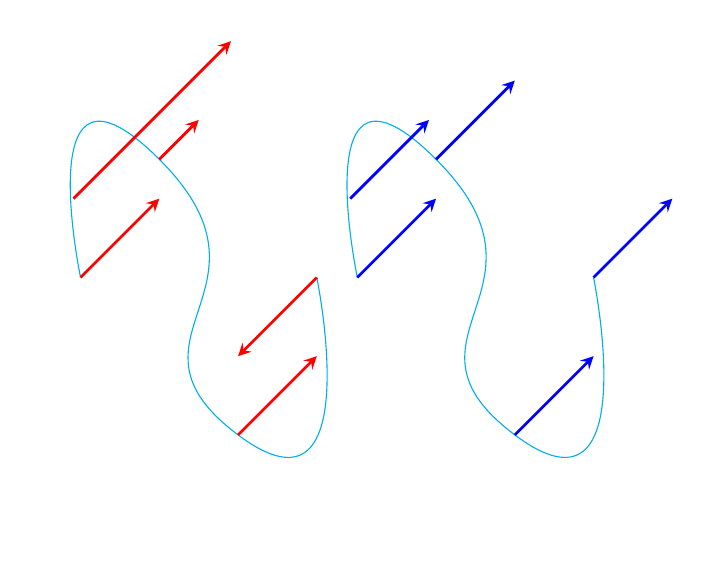
\begin{tikzpicture}
        \draw [cyan] plot [smooth, tension=3] coordinates { (0,0) (1,1.5) (2,-2) (3,0)};
        \draw[line width=1pt,blue,-stealth](0,0)--(1,1);
        \draw[line width=1pt,blue,-stealth](-0.09, 1)--(0.91,2);
        \draw[line width=1pt,blue,-stealth](1,1.5)--(2,2.5);
        \draw[line width=1pt,blue,-stealth](2,-2)--(3,-1);
        \draw[line width=1pt,blue,-stealth](3,0)--(4,1);

        \draw [cyan] plot [smooth, tension=3, xshift = -100] coordinates { (0,0) (1,1.5) (2,-2) (3,0)};
        \draw[line width=1pt,red,-stealth, xshift = -100](0,0)--(1,1);
        \draw[line width=1pt,red,-stealth, xshift = -100](-0.09, 1)--(1.91,3);
        \draw[line width=1pt,red,-stealth, xshift = -100](1,1.5)--(1.5,2.0);
        \draw[line width=1pt,red,-stealth, xshift = -100](2,-2)--(3,-1);
        \draw[line width=1pt,red,-stealth, xshift = -100](3,0)--(2,-1);
    \end{tikzpicture}
\end{center}
\begin{note}
    Explanation by Schuller:
    \begin{itemize}
        \item \textit{Parallel transport}: Pinocchio move along the curve and point your nose in the same direction always
            and \textsc{do not lie}.
        \item \textit{Parallel}: Now you're allowed to lie.
    \end{itemize}
\end{note}

\subsection{Autoparallelly Transported Curves}
\begin{defn}[Autoparallelly transported]
    A curve $\gamma: \mathbb{R} \to \M$ is called \textit{autoparallelly transported} (or just \textit{autoparallel}) if
    \begin{equation}
        \nabla_{v_\gamma} v_\gamma = 0\,.
    \end{equation}
    or (this is the same)
    \begin{equation}
        \left( \nabla_{v_{\gamma, \gamma(\lambda)}} v_\gamma \right)_{\gamma(\lambda)} = 0\,.
    \end{equation}
\end{defn}
\begin{note}
    An autoparallel curve is
    \begin{equation}
        \nabla_{v_\gamma} v_\gamma = \mu v_\gamma\,.
    \end{equation}
    even though most of the time one also uses the notion ``autoparallel'' for an autoparallelly transported curve.
    An autoparallelly transported curve is the ``straightest curve possible''.
\end{note}
\textit{Example}: \textit{Euclidean plane} $(\mathbb{R}^2, \mathcal{O}, \mathcal{A}, \nabla_E)$
Red (left): autoparallel curve, blue (right): autoparallelly transported curve.
Equal distances mean equal affine parameter $\lambda$.
\begin{center}
    \begin{tikzpicture}
        \draw[line width=1pt,blue](0,0)--(0.5,0.5);
        \draw[line width=1pt,blue](0.55,0.55)--(1,1);
        \draw[line width=1pt,blue](1.05,1.05)--(1.5,1.5);
        \draw[line width=1pt,blue](1.55,1.55)--(2,2);
        \draw[line width=1pt,blue](2.05,2.05)--(2.5,2.5);
        \draw[line width=1pt,blue](2.55,2.55)--(3.1,3.1);

        \draw[line width=1pt,red,xshift = -100](0,0)--(1,1);
        \draw[line width=1pt,red,xshift = -100](1.05,1.05)--(1.5,1.5);
        \draw[line width=1pt,red,xshift = -100](1.55,1.55)--(1.7,1.7);
        \draw[line width=1pt,red,xshift = -100](1.75,1.75)--(2.5,2.5);
        \draw[line width=1pt,red,xshift = -100](2.55,2.55)--(3.1,3.1);
    \end{tikzpicture}
\end{center}

\subsection{Autoparallel Equation} 
Let $\gamma$ be an autoparallelly transported curve.
Consider that portion of the curve that lies in $U$, where $(U,x)\in \mathcal{A}$ (atlas).
Express $\nabla_{v_\gamma}v_\gamma = 0$ (condition for the curve to be autoparallelly transported)
in terms of chart representatives:
Using $v_{\gamma, \gamma(\lambda)} = \dot{\gamma}^m_{(x)}(\lambda) \left( \frac{\partial}{\partial x^m} \right)_{\gamma(\lambda)}$
and $\gamma^m_{(x)} := x^m \circ \gamma$ we get
\begin{align}
    \nonumber \nabla_{v_\gamma}v_\gamma  &= \left( \nabla_{\dot{\gamma}^m_{(x)} \left( \frac{\partial}{\partial x^m} \right)} \dot{\gamma}^n_{(x)}  \frac{\partial}{\partial x^n}  \right)\\
    &= \underbrace{\dot{\gamma}^m \frac{\partial \dot{\gamma}^q}{\partial x^m}}_{\ddot{\gamma}^m_{(x)}} \frac{\partial}{\partial x^q} + \dot{\gamma}^m \dot{\gamma}^n \Gamma^q{}_{nm}\frac{\partial}{\partial x^q}\,.
    \label{eq:autoparallelEquation}
\end{align}
In summary we have the chart expression of the condition that $\gamma$ be autoparallelly transported:
\begin{equation}
    \boxed{%
    \ddot{\gamma}^{m}_{(x)}(\lambda) + \Gamma^m{}_{ab}(\gamma(\lambda)) \dot{\gamma}^a(\lambda)\dot{\gamma}^b(\lambda) = 0}\,.
\end{equation}
As we will see later if for $\Gamma$ we choose the so called \textit{Levi Civita connection}
then this is the \textit{geodesic equation}.

\paragraph{Examples}
\begin{enumerate}
    \item Euclidean plane:\\ $U = \mathbb{R}^d$, $x = \mathrm{id}_{\mathbb{R}^d}$, $\Gamma_(x)^{i}{}_{jl} = 0$,
        $\Rightarrow \ddot{\gamma}^m_{(x)} = 0$ $\Rightarrow \gamma_{(x)}^m(\lambda) = a^m \lambda + b^m$, $a,b\in \mathbb{R}^d$
    \item Round sphere $(S^2, \mathcal{O}, \mathcal{A}, \nabla_\text{round})$:\\
        The sphere $S^2$ as a manifold does not contain the notion of distances like we are used to from a sphere.
        Also a squished and stretched sphere is still a sphere. 
        Only when we choose a specific connection $\nabla_\text{round}$ we get what we usually see as the sphere,
        but it's actually the \textit{round sphere}.
        Consider a chart (polar coordinates)
        \begin{align}
            \nonumber x(p) &= (\theta, \phi)\,, \\
            \nonumber \theta \in (0, \pi)\,&,\quad \phi \in (0, 2\pi)\,\\
            \Gamma^1_{(x)22} (x^{-1}(\theta, \phi)) &:= - \sin\theta \cos\theta\,,\\
            \Gamma^2_{(x)21} = \Gamma^2_{(x)12} &:= \cot \theta\,.
        \end{align}
        and all other $\Gamma$s zero.
        Using sloppy notation
        \begin{align}
            x^1(p) = \theta{p}\,,
            x^2(p) = \phi(p)\,,
        \end{align}
        the autoparallel equation becomes
        \begin{align}
            \ddot \theta - \sin\theta \cos\theta\, \dot\phi \dot\phi &= 0\,,\\
            \ddot \phi + 2\cot\theta\, \dot\theta \dot\phi &= 0\,.
        \end{align}
        For example a solution is 
        \begin{align}
            \theta(\lambda) &= \pi/2 = \text{const}\,,\\
            \phi(\lambda) &= \omega \lambda + \phi_0\,.
        \end{align}
        This is a curve around the equator with constant speed.
        Similarity other curves along great circles are solutions.
\end{enumerate}
\begin{note}
    Thus if someone gives you the connection $\nabla_\text{potato}$ on a potato,
    you can calculate the straightest curves on that potato.
    Still, the potato is a 2-sphere $S^2$ as a smooth manifold.
\end{note}

\subsection{Torsion}
\begin{defn}[Commutator]
    The commutator between two vector fields $X$ and $Y$ is defined as
    \begin{equation}
        [X,Y]f := X(Y f) - Y(Xf)\,.
    \end{equation}
\end{defn}
\begin{defn}[Torsion]
    The \textit{torsion} of a connection $\nabla$ is the $(1,2)$-tensor field
    \begin{equation}
    T(\omega, X, Y) := \omega \left( \nabla_X Y - \nabla_Y X - [X,Y] \right)\,,
    \end{equation}
\end{defn}
Proof that $T$ is a tensor: Check $T$ is $C^\infty$-linear in each entry
\begin{enumerate}
    \item 
        \begin{equation}
            T(f\omega, X, Y) = f \omega (\ldots) = f T(\omega, X,Y)\,,
        \end{equation}
        \begin{align}
            T&(\omega + \psi, X, Y) = (\omega + \psi) (\ldots)\\
            \nonumber &= T(\omega, X,Y) + T(\psi, X, Y)\,,
        \end{align}
    \item
        \begin{align}
            \nonumber T&(\omega, fX, Y) = \omega \left( \nabla_{fX} Y - \nabla_Y (fX) - [fX, Y] \right)\\
            \nonumber &= \omega \left[ f\nabla_X Y - f \nabla_Y X - \cancel{(Yf)X} - fXY \right.\\
            &~\left.- fYX - \cancel{(Yf)X} \right] = f T(\omega, X, Y)\,,
        \end{align}
        where we have used
        \begin{align}
            [fX,Y]g &= fX(Yg) - Y(fXg) \\
            \nonumber &= fX(Yg) - (Yf)Xg - f(YXg)\,,
        \end{align}
        and $\nabla_Y f = Yf$.
        Since $T(\omega,X,Y) = -T(\omega, Y, X)$ we don't have to check the scaling
        in the last argument and the additivity in the middle argument also is easy.
\end{enumerate}
\begin{defn}[Torsion-free connection]
    $(\M, \mathcal{O}, \mathcal{A}, \nabla)$ is called \textit{torsion-free} if $T=0$.
    In a chart:
    \begin{equation}
        T^i{}_{ab} := T\left(\diff x^i, \frac{\partial}{\partial x^a}, \frac{\partial}{\partial x^b}\right) = 
        2\Gamma^i_{[ab]}\,.
    \end{equation}
\end{defn}
From now on we will be focusing on \textit{torsion-free} connections.

\subsection{Curvature}
\subsubsection{Riemann Curvature Tensor}
\begin{defn}[Riemann Curvature]
    The \textit{Riemann Curvature} of a connection $\nabla$ is the
    (1,3)-tensor field
    \begin{align}
        \nonumber \Riem(\omega, Z, X, Y) := w&\left( \nabla_X \nabla_Y Z - \nabla_Y\nabla_X Z \right.\\
        &-\left. \nabla_{[X,Y]}Z \right)\,.
        \label{eq:RiemannCurvature}
    \end{align}
\end{defn}
\begin{note}
    The Riemmann curvature tensor contains all information about the curvature.
    For a two-dimensional manifold the Ricci tensor is enough.
\end{note}
\begin{note}
    Of course one has to show that $\Riem$ is $C^\infty$-linear in each slot. 
    The first slot is trivial, I will show it for the second:
    \begin{align*}
         &\Riem(\omega, fZ, X, Y) := \\ 
         &=\omega\left( \nabla_X \nabla_Y (fZ) - \nabla_Y\nabla_X (fZ) - \nabla_{[X,Y]}(fZ) \right)\,.\\
         &=\omega\left[ \nabla_X( (Yf)Z) + f\nabla_Y Z) - \right.\\
         &\phantom{=}\left.\nabla_Y( (Xf)Z - f\nabla_X Z) - ([X,Y]f)Z - f\nabla_{[X,Y]}Z\right]\\
         &= \omega\left[ ( (XY - YX) f )Z + f(\nabla_X\nabla_Y - \nabla_Y\nabla_X)Z\right.\\
         &\phantom{=} \left. - ([X,Y]f)Z - f\nabla_{[X,Y]}Z\right]\\
         &= f \Riem(\omega, Z, X, Y)\,.
     \end{align*}
     The third (and by symmetry also forth) argument works the same, one just has to use
     \begin{align}
         \nonumber\nabla_{[fX,Y]}Z &= \nabla_{f[X,Y]Z - (Yf)X}Z  \\
         &=f\nabla_{[X,Y]}Z - (Yf)\nabla_X Z\,.
     \end{align}
\end{note}


\subsubsection{Algebraic Relevance of Riem}
\begin{align}
    \nonumber &\left( \nabla_X \nabla_Y - \nabla_Y \nabla_X \right)Z =\\ %cant have & in \left \right
    &\phantom{blabla}\Riem(\cdot, Z,X,Y) + \nabla_{[X,Y]}Z
\end{align}
Let's look at a chart $(U,x)$.
We write $\nabla_{\frac{\partial}{\partial x^a}} = \nabla_a$, but be careful, because when
writing it like this we throw away the information of the chart in $\nabla$.
\begin{align}
    \boxed{\left( \nabla_a\nabla_b Z \right)^m - (\nabla_b\nabla_a Z)^m = R^m{}_{nab}Z^n
    }
    \\\nonumber+ \cancel{\nabla_{[\frac{\partial}{\partial x^a},\frac{\partial}{\partial x^b}]}Z}\,,
\end{align}
where with $R^{m}{}_{nab}$ we now denote the components of $\Riem$ in the basis.
<<<<<<< HEAD

\subsubsection{Geometric Relevance of Riem}
\begin{center}
    \textsc{Put picture here of $[X,Y] = 0$ and
    $[X,Y] \neq 0$}.
    Schuller did a really god job explaining this at the end of lecture
    8, but it's hard to write down.
\end{center}

Assuming a torsion-free connection, $T=0$, then one can imagine curvature as follows.
Parallel transporting a vector $Z$ along two different paths from $p$ to $q$
changes the vector.
Going infinitesimal and ``along'' $X$ or $Y$ (first along $X$ and then along $Y$ or the other
way round) one can find (for $[X,Y] = 0$)
\begin{equation}
    (\delta Z)^m = R^m{}_{nab}X^aY^bZ^n\,\delta s\delta t\,,
\end{equation}
plus higher order terms in the ``lengths of the curves'' $\delta s$, $\delta t$.
%One contracts the first and the third index, because all others are either zero or equivalent.

